\documentclass[11pt]{report}
\usepackage{amsmath}
\usepackage{amssymb}
%\usepackage{bbm}
\usepackage{graphicx}
\usepackage{tikz}

\newcommand{\ubt}[1]{\textbf{\underline{#1}}}
\newcommand{\sps}{\\[0.2cm]}
\newcommand{\spn}[1]{\\[#1cm]}
\newcommand{\refn}[1]{(\ref{#1})}
\newcommand{\refx}[1]{\refn{eq:#1}}
\newcommand{\bt}[1]{\textbf{#1}}
\newcommand{\dsp}{\displaystyle}
\newcommand{\NI}{\noindent}
\newcommand{\real}{ \mathbb{R}}
\newcommand{\mbf}[1]{\mathbf{#1}}
\newcommand{\complex}{\mathbb{C}}
\newcommand{\sprime}{'}
\newcommand{\dprime}{''}
\newcommand{\tprime}{'''}
\newcommand{\sbracket}[1]{\left[#1\right]}
\newcommand{\example}[1]{\section*{\ubt{Example #1}}{~}\spn{-1}}
\newcommand{\examples}{\subsubsection*{Examples}{~}\spn{-1}}
\newcommand{\solution}{\subsubsection{\ubt{Solution}}{~}\spn{-1}}
\newcommand{\eg}{\subsection*{\ubt{Example}}{~}\spn{-1}}
%\newcommand{\real}{\mathbbm{R}}

\renewcommand{\baselinestretch}{1.5}
\renewcommand{\contentsname}{Table of Contents}
\renewcommand{\labelenumi}{\arabic{enumi})}
\renewcommand{\labelenumii}{\alph{enumii})}

%\setlength{\parindent}{1em}


\begin{document}
	
	%%%%%%%%%%%%%%%%%%%FRONT COVER%%%%%%%%%%%%%%%%%%%
	\addcontentsline{toc}{chapter}{TITLE PAGE}
	\clearpage
	\thispagestyle{empty}
	\begin{center}
		\Large \bt{SOLUTION OF ORDINARY DIFFERENTIAL EQUATIONS INVOLVING BIOLOGICAL SYSTEMS AND ENGINEERING PROBLEMS}
	\end{center}

	\hspace{7cm}
	
	\begin{center}
		\textbf{\textit{BY}}
	\end{center}
	
	\hspace{5cm}
	
	\begin{center}
		\large \textbf{ADELOLA, KAYODE SAMSON
			\\
			17/56EB018}
	\end{center}
	
	\hspace{9cm}
	
	\begin{center}
		A PROJECT SUBMITTED TO THE DEPARTMENT OF MATHEMATICS, FACULTY OF PHYSICAL SCIENCES, UNIVERSITY OF ILORIN, ILORIN, KWARA STATE, NIGERIA. IN PARTIAL FULFILLMENT OF REQUIREMENTS FOR THE AWARD OF BACHELOR OF SCIENCE (B. Sc.) DEGREE IN MATHEMATICS.
	\end{center}

	\hspace{7cm}
	
%	\begin{center}
%		IN PARTIAL FULFILLMENT OF REQUIREMENTS FOR THE AWARD OF BACHELOR OF SCIENCE (B. Sc.) DEGREE IN MATHEMATICS.
%	\end{center}
%	\hspace{5cm}
%	\\ \\ 
	\begin{center}
		\textbf{NOVEMBER, 2022}
	\end{center}

	\newpage
	\pagenumbering{roman}
	\addcontentsline{toc}{chapter}{CERTIFICATION}
	\section*{\begin{center}\textbf{\Large CERTIFICATION}   \end{center}}
	This is to certify that this project was carried out by \textbf{ADELOLA, Kayode Samson} with Matriculation Number  \bt{17/56EB018} in the Department of Mathematics, Faculty of Physical Sciences, University of Ilorin, Ilorin, Nigeria, for the award of Bachelor of Science (B.Sc.) degree in Mathematics.
	\\
	\\
	................................... \qquad \qquad\qquad\qquad\qquad\qquad...................... \\
	Prof. A.S. Idowu  \quad\qquad\qquad\qquad\qquad\qquad\qquad\qquad Date\\
	Supervisor\\
	\\
	\\
	\\
	...................................... \qquad\qquad\qquad\qquad\qquad\qquad ......................\\
	Prof. K. Rauf      \qquad\qquad\qquad\qquad\qquad\qquad\qquad\qquad\quad     Date\\
	Head of Department\\
	\\
	\\
	\\
	..................................... \qquad\qquad\qquad\qquad\qquad\qquad .......................\\
	Prof. T. O. Oluyo \quad\qquad\qquad\qquad\qquad\qquad\qquad\qquad         Date\\
	External Examiner 
	
	\newpage
	%%ACKNOLEDGMENTS%%
	\section*{\begin{center}\textbf{\Large ACKNOWLEDGMENTS}\end{center}}
	\addcontentsline{toc}{chapter}{ACKNOWLEDGMENTS} 			
	First and foremost, I want to give thanks and praises to Almighty God for His loving kindness and mercy for giving me the courage and determination to complete this research work.\\
	
	\NI My profound gratitude and appreciation goes to my supervisor Prof. A.S. Idowu for his useful and the valuable contribution, correction, and suggestion that greatly helps to the successful completion of this project.\\
	
	\NI My appreciation goes to my amiable and relentless Head of Department Prof. K. Rauf and my amiable Level Adviser, Dr. K. A. Bello for their words of encouragement, concern and support.\\
	
	\NI Also, my appreciation goes to all my esteem Lecturers: Prof. J. A. Gbadeyan, Prof. T. O. Opoola, Prof. O. M. Bamigbola, Prof. M. O. Ibrahim, Prof. O. A. Taiwo, Prof. R. B. Adeniyi, Prof. M. S. Dada, Prof. K. O. Babalola, Prof. A. S. Idowu, Prof. Olubunmi A. Fadipe-Joseph, Dr. E. O. Titiloye, Dr. Yidiat O. Aderinto, Dr. Catherine N. Ejieji, Dr. B. M. Yisa, Dr. J. U. Abubakar, Dr. Gatta. N. Bakare, Dr. Idayat F. Usamot, Dr. B. M. Ahmed, Dr. O. T. Olootu, Dr. O. A. Uwaheren, Dr. T. L. Oyekunle, Dr. O. Odetunde, Dr. A. Y. Ayinla and all other members of staff of the department of mathematics, who contributed greatly to my academic excellence, obtained during my period of study in the department. May God bless them all.\\
	
	\NI I am highly indebted to my loving and caring family especially my brother and sisters who have tersely contributed immensely toward the successful completion of my studies and academic activities.\\
	
	\NI To my friends inside and outside my department; big shout out to you all and thank you for your assistance and inputs during my course work and in this project. May our paths always be smooth and favour-filled. God bless you all.\\
	
	
	\newpage
	%%DEDICATION%%
	\section*{\begin{center}\textbf{\Large DEDICATION}\end{center}}
	\addcontentsline{toc}{chapter}{DEDICATION}
	This project work is dedicated to Almighty God who has brought me to this level in my undergraduate program. For His mercies, guidance and protection throughout my years of study.
	
	\newpage
	%%ABSTRACT%%
	\section*{\begin{center}\textbf{\Large ABSTRACT}\end{center}}
	\addcontentsline{toc}{chapter}{ABSTRACT}
	Differential Equations are among the most important Mathematical tools used in creating models in the science, engineering, economics, mathematics, physics, aeronautics, astronomy, dynamics, biology, chemistry, medicine, environmental sciences, social sciences, banking and many other areas.\\
	
	\NI Thus this project discusses the solutions of Ordinary Differential Equations involving Biological Systems and Engineering Problems; which is to enlightened and help students to know some various applications, examples and usefulness of differential equations in Biological Science and Engineering in general.\\ 
	
	\newpage
	%%%%%%%%%%%%%%%%%%%TABLE OF CONTENTS%%%%%%%%%%%%%%%%%%%
	\addcontentsline{toc}{chapter}{TABLE OF CONTENTS}
	\tableofcontents
	
	\newpage
	\pagenumbering{arabic}
	%%%%%%%%%%%%%%%%%%%CHAPTER ONE%%%%%%%%%%%%%%%%%%%
	\chapter{GENERAL INTRODUCTION}
	\section{HISTORICAL BACKGROUND}
	There is hardly a culture, however primitive, which does not exhibit some rudimentary kind of Mathematics, the great achievement of science and technology in all their forms which deeply influence the life of every human being has undoubtedly received great contribution from Mathematics.\\
	
	\NI In its historical development, Mathematics first proceeded in quite a nature manner, it’s started out from the number $1, 2, 3,\ldots$ and from obvious figures of geometry such as points segments lines gradually it ascended to more complex formations. Mathematics is the science of quantity and space and it also deals with the symbolism relating to quantity and the space.\\
	
	\NI Mathematics can be think of as the language of science and differential equations as one of the most important parts of this language as far as science and engineering are concerned.\\
	
	\NI Differential equation was originated by the famous Mathematicians of the seventeenth and eighteen centuries, such as Gottfried Wilhelm Leibniz (1646-1813) who made an important contribution to the theory and application of differential equations dated back to the beginning of calculus with Isaac Newton (1642-1727), Newton did a little work in the theory of differential equation, he classified first order differential equation according to the forms
	
	\begin{eqnarray}
		\frac{dy}{dx}&=&f(x)\label{eq:1_1}\sps
		\frac{dy}{dx}&=&f(y)\label{eq:1_2}\sps
		\frac{dy}{dx}&=&f(x,y)\label{eq:1_3}
	\end{eqnarray}
	For equation \refx{1_3}, he developed a method of solution using infinite series when $f(x, y)$ is a polynomial in $x$ and $y$. He was very sensitive to criticism and as a consequence he was slow in publishing many of his discoveries Leibniz arrived at the fundamental result of the calculus independently, although a little later than Newton. He discovered the method of separation of variables as well as procedures for solving first order homogenous equations and linear first order equations.\\
	
	\NI Later in the eighteenth century the great French Mathematicians Joseph Louis Lagrange (1736-1813) and Persimmon Laplace (1749-1827) made an important contribution to the theory of ordinary differential equations and gave the first scientific treatment of partial differential equation.\\
	
	\NI There are many diverse fields where differential equation is applicable, there are such area in real life and the various subject area such as in science industries, business, engineering  e.t.c.\\
	
	\NI The history of differential equation in relation to the Biology is based on growth and dynamics of population and organisms. The simplest model of population growth was first formulated by the English economist T.R Malthus in 1798. He assumed that the rate of change of a population is proportional to the size of population. If $x =x(t)$ stands for the number of individuals in the population after $t$-years, then this means.
	\begin{eqnarray}
		\frac{dx}{dt} = \lambda x \label{eq:1_4}
	\end{eqnarray}
	Where $\lambda$ is a constant. And Malthus observations on this are said to influence Darwin in his studies of species.\\
		
	\NI Differential equation is a branch of Mathematics which deals with changing quantities. It form one of the most fascinating branches of advanced Mathematics. Differential equation has hundreds of practical applications in engineering, physics, chemistry and other branch of science.\\
	
	\NI For Example; consider Newton second law of motion which state that \textit{the rate of charge of momentum is directly proportional to the force applied and take place in the direction is the applied force.} Mathematically, 
	\begin{eqnarray*}
		\frac{d(mv)}{dt} &=& F \text{ and }\sps
		\frac{dp}{dt} &=& F
	\end{eqnarray*}
	where $m$ is mass of object, $v$ is the velocity of the object, $F$ is force  and $p$ is momentum.
	
	\section{DIFFERENTIAL EQUATION}
	In mathematics, a differential equation(DE) is an equation that relates an unknown function of one or more variables and its derivatives. For instance, the equation can be written in the form. 
	\begin{eqnarray}
		y\sprime = \frac{dy}{dx} = f(x,y)\label{eq:2_1}
	\end{eqnarray}
	Subject to an initial condition $y=y_0$ at $x=x_0$. Here $y$ and $x$ are called the dependent  and independent variables respectively. In applications, the functions generally represent physical quantities, the derivatives represent their rates of change and the differential equation defines a relationship between the two.
	
	\section*{Examples of differential equations:}
	\begin{enumerate}
		\item $\dsp \frac{dx}{dt} = kx$ (Exponential growth)
		
		\item $\dsp\frac{dx}{dt} = k(A-x)$ (Newton's law of cooling)
		
		\item $\dsp m\frac{d^2x}{dt^2} +c\frac{dx}{dt} + kt = f(t)$ (Mechanical vibrations)
	\end{enumerate}
	where $k$, $A$, $m$,  and $c$ being constants
	
	
	\section{CLASSIFICATION OF DIFFERENTIAL EQUATIONS }
	Differential equation can be classified according to Types, Order, Degree and Linearity.
	
	\subsection{CLASSIFICATION BASED ON TYPES}
	There are two types of differential equation namely ordinary differential equation and partial differential equation.
	\begin{enumerate}
		\item \bt{Ordinary Differential Equation (ODE):} This is a differential equation whose dependent variable that is unknown is a function of only one independent variable. examples are:
		\begin{enumerate}
			\item $\dsp \frac{d^4y}{dx^4} - 2\frac{d^2y}{dx^2} - 3\frac{dy}{dx} - 2x = 0$
			\item $\dsp \frac{d^2y}{dt^2} - 5\frac{dy}{dt} + 6y = 2t^2 + 3 $
			\item $\dsp e^y\frac{d^2y}{dx^2} + 2\left(\frac{dy}{dx}\right)^2 = 1$
		\end{enumerate}
		
		\item \bt{Partial Differential Equation (PDE):} This is a differential equation whose dependent variables that is unknown is a function of two or more independent variables.\spn{-1.3}
		\examples
		\begin{enumerate}
			\item $\dsp \frac{\partial y}{\partial t} + c\frac{\partial y}{\partial x} = 0$
			\item $\dsp \frac{\partial u}{\partial t} = \frac{\partial^2 u}{\partial x^2}$
			\item $\dsp \frac{\partial^2 u}{\partial t^2} = \frac{\partial^2 u}{\partial x^2} + \frac{\partial^2 u}{\partial y^2}$
		\end{enumerate}
	\end{enumerate}
	
	\subsection{CLASSIFICATION BASED ON ORDER}
	This is the order of the highest derivative that appears in the equation.\spn{-1.3}
	\examples
	\begin{enumerate}
		\item $\dsp x\frac{dy}{dx} - y^2 = 0$ is an equation of the 1st order
		\item $\dsp xy\frac{d^2y}{dx^2} - y^2\sin x = 0$ is an equation of the 2nd order
		\item $\dsp\frac{d^3y}{dx^3} - y\frac{dy}{dx}+e^{4x} = 0$ is an equation of the 3rd order
	\end{enumerate}
	and so on.
	
	\subsection{CLASSIFICATION BASED ON DEGREE}
	The degree of a differential equation is that of the highest power of the highest differential which the equation contains after removing the radical sign and fraction. \spn{-1.3}
	\examples
	\begin{enumerate}
		\item $\dsp \cos x \frac{d^2 y}{dx^2} + \sin x\left(\frac{dy}{dx}\right)^2 + 8y = \tan x $ is an equation of 1st degree since the highest derivative is $\dsp \frac{d^2y}{dx^2}$ and the power is 1.
		
		\item $\dsp \frac{d^3 y}{dx^3}+ x\left(\frac{dy}{dx}\right)^{3/2} + x^2 y = 0$ is an equation of 2nd degree, since after rationalisation it contains the term $\dsp\left(\frac{d^3y}{dx^3}\right)^2$.
	\end{enumerate}
	
	
	\subsection{CLASSIFICATION BASED ON LINEARITY}
	A differential equation is said to be linear if it can be written in the form.
	\begin{multline}
		a_n(x)\frac{d^ny}{dx^n} + a_{n-1}(x)\frac{d^{n-1}y}{dx^{n-1}} + a_{n-2}(x)\frac{d^{n-2}y}{dx^{n-2}} + \cdots + a_2(x)\frac{d^2y}{dx^2} \\+ a_1(x)\frac{dy}{dx} + a_0(x)y=g(x)\label{eq:2_2}
	\end{multline}
	Where $a_j(x),~ j = 0, 1, 2, 3,\ldots n$ are known and depend on the variable $x$. if the $a_j$ are constants then the equation \refx{2_2} is called linear equation with constant coefficients. Otherwise the differential equation is non-linear. In a linear equation, if $y$ is a dependent variable, there can be no $y^2, y(dy/dt), (dy/dt)^3$ etc.\spn{-1.25}
	\examples
	\begin{enumerate}
		\item $\dsp\frac{d^2 y}{dx^2} - 3\frac{dy}{dx} + 2y = 0$ is a linear equation.
		\item $\dsp \frac{dy}{dx} + x^2\sin(y)=0$ is a non-linear equation because the dependent variable appears inside the non-linear sin operation.
	\end{enumerate}
	
	\NI To remain within the scope of this project we shall confine ourselves to the study of ordinary differential equations.
	
	
	\section{SOURCES OF ORDINARY DIFFERENTIAL EQUATIONS}
	There are two sources of differential equations
	\begin{enumerate}
		\item \bt{Mathematical formulation relationship:} Many relationships between quantities give rise to differential equation when expressed mathematically, for example many laws in physics result in differential equations. Similarly, some relationships in biology (population growth etc.) Chemistry, Medicine and so on, result in differential equations. Indeed, whenever the word ``rate'' or its equivalent is used, there is derivations and hence we have differential equations.
		
		\item \bt{Elimination of arbitrary constants:} In some cases, the relationships between some variables are given in terms of arbitrary constants. For example 
		\begin{eqnarray*}
			Z = at +bt^2
		\end{eqnarray*}
		$a$ and $b$ are constants. If we want the relationship without the constants, we have to differentiate, thus we have a differential equation. 
	\end{enumerate}
	
	\section{AIMS AND OBJECTIVES }	
	Differential equation as a discipline has retained high degree of vitality of biological, physical and social system. The aims of this project are to discipline and analyses the application of differential equation as a branch of calculus to the various field of engineering and biological science and its influence on the growth and development of these field. The objectives are to:
	\begin{enumerate}
		\renewcommand{\labelenumi}{\roman{enumi}.}
		\item explain types, methods and classification of differential equations.
		\item solve ordinary differential equations
		\item use ordinary differential equations to solve some  biological and engineering problems.
	\end{enumerate}	
		
	\section{SIGNIFICANT OF THE STUDY}
	Modern Mathematics now encompasses a vast range of topics in differential equations. This case is undoubted because of the wide variety application, ranging from the traditional area of physics, engineering to the more recent use of differential equation in biology, chemistry, economics. Biological, physical, social and engineering system are dynamics in characters, differential equation can be used to effectively analyse the evolutionary trend of such systems and in formulating of these system and the quantitative examination of their stability and adaptability external stimuli. 
	
	\section{SCOPE AND LIMITATIONS}
	This project contained some solution of some biological problems, mechanical and electrical engineering using under ordinary differential equation with constant co-efficient and it does not involve non-linear and partial differential equation.
	
	\section{STRUCTURE OF THE PROJECT}
	Chapter one provides a general introduction to differential equations including motivation with related concepts. In chapter two highlights on review of literature and methods  for solving some first order and simple higher order equations and these methods were applied in chapter three and four. In chapter three deals with some problems in biological science field and in chapter four to mechanical and electrical engineering. In the same way, chapter five consists of a summary, conclusion, recommendations and references follows.
	
		
	%%%%%%%%%%%%%%%%%%%CHAPTER TWO%%%%%%%%%%%%%%%%%%%
	\chapter{LITERATURE REVIEW}
	\section{INTRODUCTION}
	Physical problem-solving efforts progressively gave rise to mathematical models employing an equation that heavily relies on a function and its derivatives. However, a select few mathematical challenges contributed as the inspiration for the theoretical growth of this new area of mathematics, known as ordinary differential equations.\\
	 
	\NI Many if not all phenomena in biological systems and engineering are broad areas of applied mathematics involve entities which change as a function of one or more variables ranging from the movement of car along the road, the propagation of sound and wave etc. Mathematics can be think of as the language of science, and differential equation as of the most important parts of this language as far as science and engineering are concerned.\\ 
	
	\NI Differential equations can describe nearly all systems undergoing change. Differential equations and mathematical modeling can be used to study a wide range of social issues. Among the topics that have a natural fit with the mathematics in a course on ordinary differential equations are all aspects of population problems: growth of population, over-population, carrying capacity of an ecosystem, the effect of harvesting, such as hunting or fishing, on a population and how over-harvesting can lead to species extinction, interactions between multiple species populations, such as predator-prey, cooperative and competitive species. (Butcher, 2003).\\
	
	\NI The study of ``differential equations", according to British mathematician Edward Ince, and other mathematics historians is said to have begun in 1675, when German mathematician Gottfried Leibniz wrote the following equation (Arfken, 1985),
	\begin{eqnarray*}
		\int x dx = \frac{1}{2}x^2
	\end{eqnarray*}
	
	\NI In 1676, Newton solved his first differential equation. That same year, Leibniz introduced the term ``differential equations” (aequatio differentialis, Latin) or to denote a relationship between the differentials $dx$ and $dy$ of two variables $x$ and $y$(Bernoulli et al., 1894).\\
	
	\NI Swiss mathematicians, brothers Jacob Bernoulli (1654-1705) and Johann Bernoulli (1667-1748), 
	in Basel, Switzerland, were among the first interpreters of Leibniz' version of differential calculus. They were both critical of Newton's theories and maintained that Newton’s theory of fluxions was plagiarized from Leibniz' original theories, and went to great lengths, using differential calculus, to disprove Newton’s \emph{Principia}, on account that the brothers could not accept the theory, which Newton had proven, that the earth and the planets rotate around the sun in elliptical orbits. (Atkinson, 2009)\\
	
	\NI The first book on the subject of differential equations, supposedly, was Italian mathematician Gabriele Manfredi’s 1707 On the Construction of First-degree Differential Equations, written between 1701 and 1704, published in Latin.  The book was largely based or themed on the views of the Leibniz and the Bernoulli brothers. Most of the publications on differential equations and partial differential equations, in the years to follow, in the 18th century, seemed to expand on the version developed by Leibniz, a methodology, employed by those as Leonhard Euler, Daniel Bernoulli, Joseph Lagrange, and Pierre Laplace.\\
	
	\NI The search for general methods of integrating differential equations began when Isaac Newton (1642-1727) classified first order differential equations into three classes. (Adesola et al., 2015). In 1692 James Bernoulli made known the method of integrating the homogeneous differential 
	equation of the first order, and not long afterwards reduced to quadratures the problem of integrating a linear equation of the first order. (Ince, 1956)\\

	\NI In 1691 the inverse problem of tangents led Leibniz to the implicit discovery of the method of separation of variables. (Ince, 1926). However, it was John Bernoulli, in a letter to Leibniz, dated May 9, 1694, that gave us the explicit process and the term, \emph{seperatio indeterminatarum} or separation of variables. (Islam et al., 2015). But even then, in one, but important, case of: 
	\begin{eqnarray*}
		x dy - y dx = 0
	\end{eqnarray*}
	This process failed, because it led to $\dsp \frac{1}{y}dy = \frac{1}{x}dx$ and $\dsp \frac{1}{x}dx$ had not yet been integrated.\\
	
	\NI In 1696, John Bernoulli, a student, rival, and equal of his older brother James, gave a main impetus to the study of differential equations through posing his famous brachistochrone problem of finding the equation of the path down which a particle will fall from one point to another in the shortest time. (Islam et al., 2015). The equation
	\begin{eqnarray*}
		\frac{dy}{dx} + P(x)y = Q(x)y^n
	\end{eqnarray*} 
	
	\section{SOLUTION OF ORDINARY DIFFERENTIAL EQUATION}
	Solutions of ordinary differential equations (ODEs) are in general possible by different methods. The main methods of solving ordinary differential equations are analytical and numerical; all other approaches are subsets of these.\\
	
	\NI Mathematically, a \bt{solution} of Ordinary Differential Equation(ODE) on the interval $\alpha < t < \beta$ is a function $\phi$ that satisfies
	\begin{eqnarray}
		\phi^{(n)}(t) = f \left[t,\phi(t),\ldots,\phi^{(n-1)}(t)\right]\label{eq:2_3}
	\end{eqnarray}
	OR\sps
	A solution of an ordinary differential equation is a function 
	\begin{eqnarray}
		y = \phi(x)\label{eq:2_4}
	\end{eqnarray}
	that, when substituted into the equation, makes it identically zero over the interval on which the equation is defined.\sps
	It is important to note that solutions are often accompanied by intervals and these intervals can impart some important information about the solution. Consider the following example.\spn{-1.2}
	\newpage
	\example{1}
	Show that\spn{-1.3}
	\begin{eqnarray}
		y(x) = x^{-3/2}\label{eq:2_5}
	\end{eqnarray}
	 is a solution to\spn{-1.3}
	 \begin{eqnarray}
	 	4x^2 y\dprime + 12xy\sprime + 3y=0 \qquad\text{ for } x > 0\label{eq:2_6}
	 \end{eqnarray}
	{~}\spn{-1.6}
	\solution
	We need to first find the first and second derivative to the given equation \refx{2_6} using the given solution from equation \refx{2_5} i.e
	\begin{eqnarray}
		y\sprime(x) = -\frac{3}{2}x^{-5/2}\qquad \text{and} \qquad y\dprime(x) = \frac{15}{4}x^{-7/2}\label{eq:2_7}
	\end{eqnarray}
	Substituting equation \refx{2_7} for $y\dprime$ and $y\sprime$ in equation \refx{2_6}, we have
	\begin{eqnarray*}
		4x^2\left[\frac{15}{4}x^{-7/2}\right] + 12x\left[-\frac{3}{2}x^{-5/2}\right]+3\left[x^{-3/2}\right]&=&0\sps
		15x^{-3/2}-18x^{-3/2} + 3x^{-3/2} &=&0\sps
		0&=&0
	\end{eqnarray*}
	Thus, equation \refx{2_5} does satisfy the differential equation \refx{2_6} and hence is a solution. We did not use this condition $x > 0$ anywhere in the work  to show that the function would satisfy the differential equation. But recall that
	\begin{eqnarray*}
		y(x) = x^{-3/2} = \frac{1}{\sqrt{x^3}}
	\end{eqnarray*}
	In this form, it is clear that we'll nee to avoid $x=0$ at the least as this would give division by zero.
	
	\example{2}
	Shows that
	\begin{eqnarray}
		y=A\sin x +B\cos x \label{eq:2_8}
	\end{eqnarray}
	where $A$ and $B$ are two arbitrary constants is solution the Differential equation
	\begin{eqnarray}
		\frac{d^2y}{dx^2} + y = 0\label{eq:2_9}
	\end{eqnarray}
	
	\solution
	From equation \refx{2_8}, we have
	\begin{eqnarray}
		\frac{dy}{dx} = A\cos x - B\sin x\quad \text{ and } \quad \frac{d^2y}{dx^2} = -A\sin x - B\cos x \label{eq:2_10}
	\end{eqnarray}
	putting equation \refx{2_10} in equation \refx{2_9}, we have
	\begin{eqnarray*}
		-A\sin x - B\cos x + A\sin x + B\cos x &=& 0\sps
		A\sin x - A\sin x + B\cos x - B\cos x &=& 0\sps
		0 - 0 &=& 0 \sps
		0 &=& 0
	\end{eqnarray*}
	Therefore, equation \refx{2_8} satisfies the differential equation and hence is a solution to the differential equation \refx{2_9}.

	\subsection{GENERAL AND PARTICULAR SOLUTION}
	A solution to a differential equation which contains one or more arbitrary constants of integration is called the \bt{general solution} of the differential equation(i.e the set of all solutions to given differential equation). While \bt{particular solution} is any one of the solutions (i.e when additional information is given so that the arbitrary constants may be calculated and this additional information is called \bt{boundary conditions}). (Frank, 1995)
	
	\subsection{INITIAL CONDITION(S)}
	Initial Condition(s) are a condition, or set of conditions, on the solution that allow us to determine a particular solution based on the given conditions. Initial conditions (often abbreviated i.c.’s) are of the form,
	\begin{eqnarray}
		y(t_0) = y_0 \qquad \text{and/or} \qquad y^{k}(t_0) = y_k
	\end{eqnarray}
	So, in other words, initial conditions are values of the solution and/or its derivative(s) at specific points. The number of initial conditions that are required for a given differential equation depend on the order of the differential equation. 
	
	
	\subsection{INITIAL VALUE PROBLEM}
	An Initial Value Problem (or IVP) is a differential equation along with an appropriate number of initial conditions. The following are examples of Initial Value Problem(IVP)
	\begin{enumerate}
		\item $\dsp 4x^2y\dprime + 12xy\sprime + 3y =0\qquad y(4)=\frac{1}{8},\quad y\sprime(4)=-\frac{3}{64}$
		\item $\dsp 2ty\sprime(t) + 4y(t) = 3\qquad y(1)=-4$
	\end{enumerate}


	\section{METHOD OF SOLUTION}
	There are variety of methods of solving ordinary differential equations. Some of which are Analytical method, Graphical method and Numerical method. This project is interested in solving ordinary differential equations, using some analytical method. 
	
	\subsection*{Common Questions}
	\begin{enumerate}
		\item \bt{(Existence)} Does a solution exist? Not all Initial Value Problems(IVP) has solutions.
		\item \bt{(Uniqueness)} If a solution exists how many are there? There can be none, one or infinitely many solution to an IVP.
		\item How can we find the solution(s) if they exist? This is the key question in this chapter. This chapter will discussed some analytical methods for solving ordinary differential equations.
	\end{enumerate}
	
	\NI Hence the following methods for solving first order differential equations will be considered. 
	
	\subsection{SEPARABLE EQUATIONS}
	A differential equation is said to be \bt{Separable} if it can be written in the form $M(x) + N(y)\frac{dy}{dx}=0$ where $M(x)$ is a function of $x$ and $N(y)$ is a function of y.\sps
	In general, we want to solve first order differential equations of the form
	\begin{eqnarray}
		\frac{dy}{dx} = f(x,y)\label{eq:2_11}
	\end{eqnarray}
	We begin with equations that have a special form referred to as \bt{separable} equations of the form
	\begin{eqnarray}
		\frac{dy}{dx} = f(y)g(x)\label{eq:2_12}
	\end{eqnarray}
	where $f(x)$ and $g(y)$ are functions of $x$ and $y$ respectively, including cases in which $f(x)$ or $g(y)$ is simply a constant. Rearranging this equation so that the terms depending on $x$ and on $y$ appear on opposite sides and equation \refx{2_12} can be written in the form of
	\begin{eqnarray}
		f(y)dy = g(x)dx
	\end{eqnarray}
	 Thus, we say that variables are separable and we get the solution by integrating both sides.
	
	\subsubsection{The General Solution Method}
	\begin{enumerate}
		\renewcommand{\labelenumi}{Step \arabic{enumi}:}
		\item (Separate) i.e $\dsp f(y)dy = g(x)dx$
		
		\item (Integrate) i.e $\dsp\int f(y)dy = \int g(x)dx$
		
		\item (Solve for $y$ and add an arbitrary constant $c$ on the right and side) i.e $F(y) = G(x) + c$
	\end{enumerate}
	
	\example{1}
	Solve\spn{-1.3}
	\begin{eqnarray}
		\frac{dy}{dx} = (1+x)(1+y)\label{eq:2_15}
	\end{eqnarray}
	
	\solution
	By separating the variables, we can rewrite equation \refx{2_15} as
	\begin{eqnarray}
		(y+1)\frac{dy}{dx} = 2x\label{eq:2_16}
	\end{eqnarray}
	Now integrate both sides of \refx{2_16} with respect to $x$ i.e
	\begin{eqnarray*}
		\int (y+1)\frac{dy}{dx}dx &=& \int 2x dx\sps
		\int (y+1)dy &=& \int 2x dx\sps
	\end{eqnarray*}
	And this gives us
	\begin{eqnarray*}
		\frac{y^2}{2} + y = x^2 + c
	\end{eqnarray*}
	which is the general solution to \refx{2_15}
	
	\example{2}
	Solve\spn{-1.3}
	\begin{eqnarray}
		\frac{dy}{dx} = \frac{y^2 + xy^2}{x^2y - x^2}\label{eq:2_17}
	\end{eqnarray}
	
	\solution
	First, by expressing the the right hand side of equation \refx{2_17} in `x-factors' and `y-factors' we have
	\begin{eqnarray}
		\frac{dy}{dx} = \frac{y^2(1+x)}{x^2(y-1)}\label{eq:2_18}
	\end{eqnarray}
	Now, separating the variables i.e rearranging the equation \refx{2_18} so that we we have `y-factors' and $dy$ on the left hand side and the `x-factors' and $dx$ on the right hand side, we have
	\begin{eqnarray}
		\frac{y-1}{y^2}dy = \frac{1+x}{x^2}dx\label{eq:2_19}
	\end{eqnarray}
	Integrating both sides of \refx{2_19} gives
	\begin{eqnarray*}
		\int\frac{y-1}{y^2}dy &=& \int\frac{1+x}{x^2}dx\sps
		\int\left\{\frac{1}{y} - y^{-2}\right\}dy &=& \int\left\{x^{-2} + \frac{1}{x}\right\}dx\sps
		\ln y + y^{-1} &=& \ln x - x^{-1} + c\sps
		\ln y + \frac{1}{y} &=& \ln x - \frac{1}{x} + c
	\end{eqnarray*}
	
	\example{3}
	Solve the equation\spn{-1.2} 
	\begin{eqnarray}
		\frac{d\theta}{dt}=2e^{3t-2\theta}\label{eq:2_20}
	\end{eqnarray}
	subject to the initial condition\spn{-1.2}
	\begin{eqnarray}
		\theta(0) = 0\label{eq:2_21}
	\end{eqnarray}
	{~}\spn{-2}
	
	\solution
	By the laws of indices, equation \refx{2_20} can be rewritten as 
	\begin{eqnarray}
		\frac{d\theta}{dt} = 2e^{3t-2\theta} = 2\big(e^{3t}\big)\big(e^{-2\theta}\big)\label{eq:2_22}
	\end{eqnarray}
	Separating the variables in \refx{2_22} gives
	\begin{eqnarray}
		\frac{d\theta}{e^{-2\theta}} &=& 2e^{2t}dt\notag\sps
		e^{2\theta}d\theta &=&2e^{3t}dt\label{eq:2_23}
	\end{eqnarray}
	Integrating both sides of equation \refx{2_23} gives
	\begin{eqnarray*}
		\int e^{2\theta}d\theta &=&\int 2e^{3t}dt
	\end{eqnarray*}
	Thus the general solution is
	\begin{eqnarray}
		\frac{1}{2}e^{2\theta} = \frac{2}{3}e^{3t} + c\label{eq:2_24}
	\end{eqnarray}
	which is the general solution to \refx{2_20}. Now, using the given condition \refx{2_21} in equation \refx{2_24}, i.e when $t=0$, $\theta=0$, thus we have
	\begin{eqnarray*}
		\frac{1}{2}e^{0} &=& \frac{2}{3}e^{0} + c\sps
		c &=& \frac{1}{2} - \frac{2}{3}\sps
		c & =& = -\frac{1}{6}
	\end{eqnarray*}
	Hence, the particular solution to \refx{2_20} is given by
	\begin{eqnarray*}
		\frac{1}{2}e^{2\theta} &=& \frac{2}{3}e^{3t} - \frac{1}{6} \quad \text{ or } \sps
		3e^{2\theta} &=&4e^{3t} - 1
	\end{eqnarray*}
	
	\subsection{HOMOGENEOUS DIFFERENTIAL EQUATIONS}
	A differential equation of the form
	\begin{eqnarray}
		f(x,y)dy &=& \varphi(x,y)dx\\
		\frac{dy}{dx} &=& \frac{f(x,y)}{\varphi(x,y)}\label{eq:2_26}
	\end{eqnarray}
	is said to be homogeneous equation if each term of $f(x,y)$ and $\varphi(x,y)$ is of the same degree i.e., $\dfrac{xy + y^3}{x^2 + xy}$. In such case, we put
	\begin{eqnarray}
		y = vx \quad\text{ and }\quad \frac{dy}{dx} = v + x\frac{dv}{dx}
	\end{eqnarray}
	and this reduces \refx{2_26} which involves only $v$ and $x$. This new differential equation can now be solved using variables separable method as discussed in the previous section.
	
	\subsubsection*{Working Rule for solving Homogeneous Differential Equations}
	\bt{Step 1:} Substitute  $y = vx$ in the given differential equation.\sps
	\bt{Step 2:} Differentiating, so that, $\dfrac{dy}{dx} = v + x\dfrac{dv}{dx}$.\sps
	\bt{Step 3:} Separating the variables and Integrate both the sides.\sps
	\bt{Step 4: } Lastly, transform the variables back to $x$ and $y$ by putting $v = \dfrac{y}{x}$ and simplify.
	
	\example{1}
	Solve the homogenous equation
	\begin{equation*}
		(y^2 + xy)dx - x^2dy = 0
	\end{equation*}
	
	\solution
	Rearranging the given differential equation, we have
	\begin{equation}
		\frac{dy}{dx} = \frac{(y^2 + xy)}{x^2}\tag{1}\label{t:t_1_1}
	\end{equation}
	Substituting $y=vx$ and $\dfrac{dy}{dx} = v + x\dfrac{dv}{dx}$ into \refn{t:t_1_1}, we have
	\begin{eqnarray*}
		v + x\frac{dv}{dx} &=& \frac{\left((vx)^2 + x(vx)\right)}{x^2}\sps
		v + x\frac{dv}{dx} &=& \frac{v^2x^2 + vx^2}{x^2}\sps
		v + x\frac{dv}{dx} &=& v^2 + v\sps
		x\frac{dv}{dx} &=& v^2
	\end{eqnarray*}
	Using variable separable method, we have
	\begin{eqnarray*}
		\int\frac{1}{v^2}dv &=& \int\frac{1}{x}dx\sps
		\int v^{-2}dv &=& \int \frac{1}{x}dx\sps
		-\frac{1}{v} &=&\ln x + \ln A\sps
		-\frac{1}{v} &=& \ln(xA)
	\end{eqnarray*}
	Now, substitute $v=\frac{y}{x}$, we get
	\begin{eqnarray*}
		-\frac{1}{\frac{y}{x}} &=& \ln(xA)\sps
		-\frac{x}{y} &=& \ln(xA)\sps
		e^{-x/y} &=& xA\sps
		x &=& A_1e^{-x/y}
	\end{eqnarray*}
	where $A_1 = \dfrac{1}{A}$
	
	\example{2}
	Solve the following differential equation
	\begin{eqnarray*}
		(2xy + x^2)\frac{dy}{dx} = 3y^2 + 2xy
	\end{eqnarray*}
	
	\solution
	We have
	\begin{eqnarray*}
			(2xy + x^2)\frac{dy}{dx} &=& 3y^2 + 2xy\sps
			\frac{dy}{dx} &=& \frac{3y^2 + 2xy}{2xy + x^2}
	\end{eqnarray*}
	substituting $y=vx$ so that $\dfrac{dy}{dx}=v + x\frac{dv}{dx}$, the given equation becomes
	\begin{eqnarray*}
		v + x\frac{dv}{dx} &=& \frac{3v^2 x^2 + 2vx^2}{2vx^2 + x^2}\sps
		v + x\frac{dv}{dx} &=& \frac{3v^2 + 2v}{2v + 1}\sps
		x\frac{dv}{dx} &=& \frac{3v^2 + 2v - 2v^2 - v}{2v + 1}\sps
		x\frac{dv}{dx} &=& \frac{v^2 + v}{2v + 1}
	\end{eqnarray*}
	Separating the variables and solve, we have
	\begin{eqnarray*}
		\left(\frac{2v+1}{v^2+1}\right)dv &=& \frac{1}{x}dx\sps
		\int\left(\frac{2v+1}{v^2+1}\right)dv &=& \int \frac{1}{x}dx\sps
		\ln(v^2 + v) &=& \ln(x) + \ln(A)\sps
		\ln(v^2+v) &=& \ln(xA)\sps
		v^2+v = Ax
	\end{eqnarray*}
	Putting $v = \dfrac{y}{x}$, we have
	\begin{eqnarray*}
		\frac{y^2}{x^2} + \frac{y}{x} = Ax\sps
		y^2 + xy = Ax^3
	\end{eqnarray*}
	
	\subsection{LINEAR DIFFERENTIAL EQUATIONS}
	A differential equation of the form
	\begin{eqnarray}
		\frac{dy}{dx} + P(x)y = Q(x) \label{eq:2_28}
	\end{eqnarray}
	is called a linear differential equation. In this case, we multiply both side of \refx{2_28} by $\dsp e^{\int P(x)dx}$ that is
	\begin{eqnarray}
		e^{\int P(x)dx}\left(\frac{dy}{dx} + P(x)y\right)= Q(x)e^{\int P(x)dx}\label{eq:2_29}
	\end{eqnarray}
	The left hand side of \refx{2_29} is exactly 
	\begin{eqnarray*}
		\frac{d}{dx}\left(y\cdot e^{\int P(x)dx} \right)
	\end{eqnarray*}
	Thus, equation \refx{2_28} becomes
	\begin{eqnarray}
		\frac{d}{dx}\left(y\cdot e^{\int P(x)dx} \right) = Q(x)e^{\int P(x)dx}\label{eq:2_30}
	\end{eqnarray}
	Integrating both sides of \refx{2_30}, we have
	\begin{eqnarray*}
		y\cdot e^{\int P(x)dx} = \int Q(x)\cdot e^{\int P(x)dx} dx + C
	\end{eqnarray*}
	Which is the required solution and $e^{\int P(x)dx}$ is called the integrating factor.
	
	\example{1}
	Solve
	\begin{eqnarray*}
		(x+1)\frac{dy}{dx} - y = e^{x}(x+1)^2
	\end{eqnarray*}
	
	\solution
	Rearranging, we get
	\begin{eqnarray*}
		\frac{dy}{dx}  - \frac{y}{x+1} = e^{x}(x+1)
	\end{eqnarray*}
	Here,
	\begin{eqnarray*}
		P(x) = -\frac{1}{x+1} \qquad \text{and}\qquad Q(x) = e^x(x+1)
	\end{eqnarray*}
	Now, finding the integrating factor, we have
	\begin{eqnarray*}
		e^{-\int\frac{1}{x+1}dx} = e^{\ln(x+1)} = e^{\ln(x+1)^{-1}} = \frac{1}{x+1}
	\end{eqnarray*}
	Thus, the solution of the differential equation is given by
	\begin{eqnarray*}
		y \cdot \frac{1}{x+1} &=& \int e^x \cdot (x+1) \cdot \frac{1}{x+1} dx\sps
		y \cdot \frac{1}{x+1} &=& \int e^x dx\sps
		\frac{y}{x+1} &=& e^x + C 
	\end{eqnarray*}
	
	\example{2}
	Solve the following first order DE
	\begin{eqnarray*}
		\frac{dy}{dx} +\left(\frac{1+x}{x}\right)y = \frac{e^x}{x}
	\end{eqnarray*}
	
	\solution
	Here, we have
	\begin{eqnarray*}
		P(x) = \frac{1+x}{x}\qquad \text{and}\qquad Q(x) = \frac{e^x}{x}
	\end{eqnarray*}
	and the integrating factor is given by
	\begin{eqnarray*}
		IF &=& e^{\int\frac{1+x}{x}dx}\\
		&=& e^{\left(\frac{1}{x} + 1\right)dx}\\\
		&=& e^{(\ln x + x)}\\
		&=& e^{\ln x} \cdot e^{x}\\
		&=& xe^x
	\end{eqnarray*}
	Thus the generation solution is given 
	\begin{eqnarray*}
		xe^xy &=& \int(xe^x)\left(\frac{e^x}{x}\right)dx\sps
		xe^xy &=& \int e^{2x}dx\sps
		y &=& \frac{1}{dxe^x}\left[\frac{e^{2x}}{2} + C\right]\sps
		y &=& \frac{e^x}{2x} + \frac{C}{xe^x}
	\end{eqnarray*}
	
	\subsection{EXACT DIFFERENTIAL EQUATIONS}
	The next type of first order differential equations that we’ll be looking at is exact differential equations.\sps
	An exact differential equation is formed by directly differentiating its solution without any other process such that
	\begin{eqnarray}
		Mdx + Ndy = 0
	\end{eqnarray}
	is said to be an exact differential equation if it satisfies the following condition
	\begin{eqnarray}
		\frac{\partial M}{\partial y} = \frac{\partial N}{\partial x}
	\end{eqnarray}
	\subsubsection*{Method for solving Exact Differential Equations}
	\bt{Step 1:} Integrate $M$ w.r.t $x$ keeping $y$ constant.\\
	\bt{Step 2:} Integrate only the term in $N$ which do not contain x w.r.t $y$ \\
	\bt{Step 3:} Setting Step 1 result + Step 2 result = Constant.\\
	
	\example{1}
	Solve
	\begin{eqnarray*}
		(5x^4 + 3x^2y^2 - 2xy^3)dx + (2x^3y-3x^2y^2 - 5y^4)dy = 0
	\end{eqnarray*}

	\solution
	From the above DE, we have $M=5x^4 + 3x^2y^2 - 2xy^3$ and $N=2x^3y - 3x^2y^2 - 5y^4$.\sps
	Now, testing for exactness, we have
	\begin{eqnarray*}
		\frac{\partial M}{\partial y} = 6x^2 - 6xy^2 \qquad\text{and}\qquad \frac{\partial N}{dx} = 6x^2y-6xy^2
	\end{eqnarray*}
	Thus, the given DE is exact and the general solution is given by
	\begin{eqnarray*}
		\int Mdx + \int (\text{terms of $N$ not containing x})dy = C\sps
		\int(5x^4+3x^2y^2 - 2xy^3)dx + \int(-5y^4)dy = C\sps
		x^5 + x^3y^2 - x^2y^3 - y^5 = C
	\end{eqnarray*}
	
	\example{2}
	Show that the following equation is exact and find its general solution
	\begin{eqnarray*}
		\left(2xy\cos x^2 - 2xy + 1\right)dx + \left(\sin x^2 - x^2 + 3\right)dy = 0
	\end{eqnarray*}

	\solution
	Comparing the given DE with $Mdx + Ndy = 0$, we have
	\begin{eqnarray*}
		M = 2xy\cos x^2 - 2xy + 1 \qquad\text{and}\qquad \frac{\partial M}{\partial y} = 2x\cos x^2 - 2x\sps
		N = \sin x^2 - x^2 -3 \qquad\text{and}\qquad \frac{\partial N}{\partial x} = 2x\cos x^2 - 2x
	\end{eqnarray*}
	Here, $\dfrac{\partial M}{\partial y} = \dfrac{\partial N}{\partial x}$ thus, the given DE is exact differential equation. The general solution is given by
	\begin{eqnarray*}
		\int Mdx + \int (\text{terms of $N$ not containing x})dy = C\sps
		\int (2xy\cos x^2 - 2xy + 1) dx + \int 3dy = C\sps
		y\int 2x \cos x^2 dx - 2y\int x dx + \int dx+ 3\int dy = C\sps 
	\end{eqnarray*}
	using $x^2 = t$ so that $2xdx = dt$, thus we have
	\begin{eqnarray*}
		y\int \cos t dt - 2y\int x dx + \int dx+ 3\int dy = C\sps
		y\sin t - x^2 y + x + 3y = C\sps
		y\sin x^2 - yx^2 + x + 3y = C
	\end{eqnarray*}
	
	
	\subsection{BERNOULLI EQUATIONS}
	In this section we are going to take a look at differential equations in the form,
	\begin{eqnarray}
		\frac{dy}{dx} + P(x)y = Q(x)y^n\label{eq:2_33}
	\end{eqnarray}
	where $P(x)$ and $Q(x)$ are continuous functions on the given interval and $n$ is a real number. Differential equations in this form are called \bt{Bernoulli Equations}.\sps
	If $n=0$, the equation becomes a linear differential equation. In case of $n=1$, the equation becomes separable. In general case, when $n\neq 0,1$, Bernoulli equation can be converted to a linear differential equation using the change of variable.
	
	\NI In order to solve \refx{2_33} we'll first divide through the equation by $y^n$ to get,
	\begin{eqnarray}
		y^{-n}\frac{dy}{dx} + P(x)y^{1-n} = Q(x)\label{eq:2_34}
	\end{eqnarray}  
	Now, using the substitution
	\begin{eqnarray}
		v = y^{1-n}\label{eq:2_35}
	\end{eqnarray}
	to convert \refx{2_34} into a differential equation in terms of $v$ which lead to a differential equation that can be solve easily.\sps
	Differentiating both sides of \refx{2_35} with respect to $x$ and noting that $v$ is a function of $x$, we have
	\begin{eqnarray}
		\frac{dv}{dx} = (1-n)y^{n}\frac{dy}{dx}\label{eq:2_36}
	\end{eqnarray}
	Now, plugging \refx{2_36} into \refx{2_34}, we have
	\begin{eqnarray}
		\frac{1}{1 - n}\frac{dv}{dx} + P(x)v = Q(x)\label{eq:2_37}
	\end{eqnarray}
	Equation \refx{2_37} is a linear differential equation that can be solve for $v$ and get the solution to the original differential equation by plugging back the value of $v$ using the equation \refx{2_35} for $y$.
	
	\example{1}
	Solve the differential equation
	\begin{equation}
		\frac{dy}{dx} + \frac{y}{x} = y^2\tag{1}\label{ex:t_1_1}
	\end{equation}
	
	\solution
	As it can be seen, this differential equation is a Bernoulli equation. To solve it, we make the substitution
	\begin{equation}
		v = y^{1-n}\tag{2}\label{ex:t_1_2}
	\end{equation}
	Here, $n=2$. From \refn{ex:t_1_2}, we have
	\begin{equation}
		v = y^{1-2} = y^{-1}= \frac{1}{y}\tag{3}\label{ex:t_1_3}
	\end{equation}
	Differentiating \refn{ex:t_1_3}, we get
	\begin{equation}
		\frac{dv}{dx} = -\frac{1}{y^2}\frac{dy}{dx}\tag{4}\label{ex:t_1_4}
	\end{equation}
	Dividing the original \refn{ex:t_1_1} by $y^2$, we have
	\begin{equation}
		\frac{1}{y^2}\frac{dy}{dx} + \frac{1}{yx} = 1\tag{5}\label{ex:t_1_5}
	\end{equation}
	using \refn{ex:t_1_3} and \refn{ex:t_1_3} in \refn{ex:t_1_5}, we get
	\begin{gather*}
		\frac{dv}{dx} - \frac{v}{x} = -1
	\end{gather*}
	We get the linear equation for the function of $v(x)$, so we the differential equation can now be solved using the integrating factor technique.\sps
	Here, $P(x) = -\frac{1}{x}$ and $Q(x)=-1$, thus the integrating factor is given by
	\begin{eqnarray*}
		IF = e^{-\int\frac{dx}{x}} = e^{-\ln x} = e^{\ln(\frac{1}{x})} = \frac{1}{x}
	\end{eqnarray*}
	Hence, the general solution for $v(x)$ is given by
	\begin{eqnarray*}
		v &=& x\left[-1\int\frac{1}{x}dx\right]\sps
		v &=& x(C-\ln(x))
	\end{eqnarray*}
	Now, making the substitution for $v = \frac{1}{y}$, we have
	\begin{eqnarray*}
		y = \frac{1}{x(C-\ln(x))}
	\end{eqnarray*}
	which is the required solution to the given differential equation.

	\example{2}
	Find the solution of the differential equation
	\begin{equation}
		4xy\frac{dy}{dx} = y^2 + x^2\tag{1}\label{ex:t_2_1}
	\end{equation}
	satisfying the initial condition $y(1)=1$.

	\solution
	Rearranging and dividing through equation \refn{ex:t_2_1}, we get
	\begin{equation}
		\frac{dy}{dx}  - \frac{y}{4x} = \frac{x}{4y}\tag{2}\label{ex:t_2_2}
	\end{equation}
	Here, $n=-1$, thus we have
	\begin{equation}
		v = y^{1-n} = y^2\tag{3}\label{ex:t_2_3}
	\end{equation}
	Differentiating, we get
	\begin{equation}
		\frac{dv}{dx} = 2y\frac{dy}{dx}\tag{4}\label{ex:t_2_4}
	\end{equation}
	multiply both sides of \refn{ex:t_2_2}, we get
	\begin{equation}
		2y\frac{dy}{dx} - \frac{y^2}{2x} = \frac{x}{2}\tag{5}\label{ex:t_2_5}
	\end{equation}
	Now, using \refn{ex:t_2_3} and \refn{ex:t_2_4} in \refn{ex:t_2_5}, we have
	\begin{eqnarray*}
		\frac{dv}{dx} - \frac{1}{2x}v = \frac{x}{2}
	\end{eqnarray*}
	Here, $P(x) = -\frac{1}{2x}$ and $Q(x)=\frac{x}{2}$, thus the integrating factor is given by
	\begin{eqnarray*}
		IF = e^{-\frac{1}{2}\int\frac{dx}{x}} = e^{-\frac{1}{2}\ln x} = e^{\ln(\frac{1}{\sqrt{x}})} = \frac{1}{\sqrt{x}}
	\end{eqnarray*}
	The general solution in term of $v(x)$ is given by
	\begin{eqnarray*}
		v &=& \sqrt{x}\left[\int \left(\frac{x}{2} \cdot \frac{1}{\sqrt{x}}\right)dx\right] \sps
		v &=& \sqrt{x}\left[\frac{1}{2}\int \sqrt{x}dx\right]\sps
		v &=& \sqrt{x}\left[\frac{1}{2}\cdot \frac{2x^{3/2}}{3}+C\right]\sps
		v & =& \frac{x^2}{3} + C\sqrt{x}
	\end{eqnarray*}
	Now, making equation in term of $y$ noting that $z=y^2$, we have
	\begin{eqnarray*}
		y = \pm\sqrt{\frac{x^2}{3} + C\sqrt{x}}
	\end{eqnarray*}
	Using the giving initial condition $y(1)=1$, we have
	\begin{eqnarray*}
			1 &=& \sqrt{\frac{1^2}{3} + C\sqrt{1}} \sps
			1 &=& \sqrt{\frac{1}{3} + C}\sps
			1 &=& \sqrt{\frac{1+3C}{3}}\sps
			1^2 &=& \frac{1+3C}{3}\sps
			3 &=& 1+3C\sps
			C &=& \frac{2}{3}
	\end{eqnarray*}
	So the solution of the IVP is given by the function
	\begin{eqnarray*}
			y = \pm\sqrt{\frac{x^2 + 2\sqrt{x}}{3}}
	\end{eqnarray*}

	
	%%%%%%%%%%%%%%%%%%%CHAPTER THREE%%%%%%%%%%%%%%%%%%%
	\chapter{APPLICATIONS INVOLVING BIOLOGICAL SCIENCE}
	\section{INTRODUCTION}
	This chapter contains some application of first order differential equation in Biological sciences. Different biological systems can be described and modelled mathematically using ordinary differential equation. \\

	\NI Although the chapter will contain only a few fields of applications but all the areas covered are of important not only to Biologist, it covered some important medical problems that are solved using differential equation.

	\section{POPULATION GROWTH AND DYNAMICS}
	All continuous population models make the basis assumption that the dynamic of a closed population, whose size is denoted by $N(t)$ are described by a differential equation of the form.
	\begin{eqnarray}
		\frac{dN(t)}{dt} = R(t,N)N
	\end{eqnarray} 
	
	mathematical population dynamics deals with techniques and methods of solving and/or analysing time behaviour of models describing populations of living entities, ranging from cells or bacteria (or even genes) through plants, animals to humans. The description can be stochastic or deterministic at the individual, population, or community level.\\
	
	\NI One of the most prevalent applications of exponential functions involves growth and decay models. Exponential growth and decay show up in a host of natural applications. From population growth and continuously compounded interest to radioactive decay and Newton’s law of cooling, exponential functions are ubiquitous in nature. In this section, we examine exponential growth and decay in the context of some of these applications.

	\subsection{EXPONENTIAL GROWTH AND DECAY}
	Let ``N" be the size of the population of some objects and ``t" be the independent variable (normally time) during which the variation and the changes in ``N" are measured. We assumed that both birth and death are proportional to the population size and the time interval. That is, mathematical terms we have. 
	\begin{eqnarray}
		\text{Birth} = \beta N dt
	\end{eqnarray}
	where $\beta$ is a constant of proportionality, $dt$ is the change in term and $N$ is the size of population.\\
	
	\NI Similarly,
	\begin{eqnarray}
		\text{Death} = \beta N dt
	\end{eqnarray}
	Let $dN$ denotes the increase of total population in the time interval $dt$. From the two expressions, we have
	\begin{eqnarray}
		dN &=& \beta Ndt - \delta N dt\notag\sps
		dN &=& N(\beta-\delta)dt\notag\sps
		dN &=& \lambda N dt\label{eq:3_4}
	\end{eqnarray}
	Where $\lambda = (\beta-\delta)$. After separating the variables, to get $N$ we can now solve the first order differential equation \refx{3_4} as follows
	\begin{eqnarray}
		\frac{1}{N}\frac{dN}{dt} &=& \lambda\notag\sps
		\int\frac{dN}{N} &=& \lambda dt\notag\sps
		\ln(N) &=& \lambda t + \ln N_0\notag\sps
		\ln N - \ln N_0 &=& \lambda t \label{eq:3_5}
	\end{eqnarray}
	Taking the exponential of both sides of equation \refx{3_5} and rearranging, we have
	\begin{eqnarray}
		N = N_0 e^{\lambda t}\label{eq:3_6}
	\end{eqnarray}
	Hence, from equation \refx{3_6}
	\begin{enumerate}
		\renewcommand{\labelenumi}{\arabic{enumi}).}
		\item If $\lambda>0$, we have exponential growth
		\item  If $\lambda < 0$, we have exponential decay
		If $\lambda=0$, we have constant growth (no change in population size).
	\end{enumerate}
	
	\example{1}
	A sample culture medium contains approximately 500 bacteria when first measured, and 72 minutes later the number has doubled to 1000.\sps
	(a)Determine a formula for the number $N(t)$ at any time $t$ hours after the initial measurement.\\
	(b)What is the number of bacteria at the end of 3hours?\\
	(c)How long does it take for the number ot increase tenfold to 5000?
	
	\solution
	\begin{enumerate}
		\renewcommand{\labelenumi}{(\alph{enumi})}
		\item When $t = 1.2$, equation \refx{3_6} becomes
			\begin{eqnarray*}
				1000 = 500e^{k(1.2)}
			\end{eqnarray*}
			dividing through by 500, and take the natural logarithm of both sides, and solve for $k$, we have
			\begin{eqnarray*}
				2 = e^{1.2k}\sps
				\ln 2 = \ln e^{1.2k}\sps
				1.2k = \ln2\sps
				k=\frac{\ln 2}{1.2}\sps
				k \approx 0.578
			\end{eqnarray*}
			Thus,
			\begin{equation}
				N(t) = 500e^{0.578t}\tag{i}\label{eq:ex:1_1}
			\end{equation}
		\item When $t=3$, $N(3) = 500e^{0.578(3)}=500e^{1.734} \approx 2832$, so at the end of 3 hours, there are approximately 28000 bacteria in the culture.
		\item To find $t$ when $N(t)=5000$, we substitute 5000 for $N(t)$ in \refn{eq:ex:1_1} and solve for $t$, we have
		\begin{eqnarray*}
			5000 &=& 500e^{0.578t}\sps
			10 &=& e^{0.578t}\sps
			\ln 10 &=& \ln e^{0.578t} = 0.578t \sps
			t &=& \frac{\ln 10}{0.578} \approx 3.98
		\end{eqnarray*}
		It takes about 4 hours for the number of bacteria to increase tenfold.
	\end{enumerate}

	\example{2}
	The half-life of carbon-14 is 5,730 years. Find the exponential decay model of carbon-14. Solve it by using the exponential decay formula and round the proportionality constant to 4 decimals
	
	
	\solution
	Using the given data, we can say that carbon-14 is decaying and hence we use the formula of exponential decay
	\begin{equation*}
		N(t) = N_0e^{-kt}
	\end{equation*}
	Here, $N_0$ = initial amount of carbon\sps
	It is given that the half-life of carbon-14 is 5,730 years. It means $N(t) = \frac{N_0}{2}=$Half of the initial amount of carbon when $t=5,730$.\sps
	Substituting all these values in the formula of exponential decay, we have
	\begin{eqnarray*}
		\frac{N_0}{2} = N_0 e^{k(5730)}
	\end{eqnarray*}
	Dividing both sides by $N_0$
	\begin{equation*}
		0.5 = e^{-k(5730)}
	\end{equation*}
	Taking logarithm of both sides,
	\begin{eqnarray*}
		\ln 0.5 = -5730k
	\end{eqnarray*}
	Dividing both sides by -5730,
	\begin{eqnarray*}
		k = \ln\left(\frac{0.5}{-5730}\right) \approx 1.2097
	\end{eqnarray*}
	Thus, the exponential decay model of carbon-14 is 
	\begin{eqnarray*}
		N(t) = N_0e^{-1.2097k}
	\end{eqnarray*}


	\section{EPIDEMIOLOGY (SPREAD OF DISEASES IN POPULATION)}
	The rate of the spread of disease (rumours) in a population is proportional to the product of the infected people and uninfected. Let $S$ be the total population of certain animals and $R$ be the number of animals that are affected by a particular disease at time $t$. Suppose $C$ is the number of animals who are not affected by the diseases. Then $C$ can be written as $C = (S – R)$. Therefore,
	\begin{eqnarray}
		\frac{dR}{dt} = KR(S-R)\label{eq:3_7}
	\end{eqnarray}
	where $K$ is a constant of proportionality. Equation \refx{3_7} can be solved by separation of variables.
	\begin{eqnarray}
		\int\frac{1}{R(S-R)}dR = \int Kdt\label{eq:3_8}
	\end{eqnarray}
	Consider the LHS of \refx{3_8}, 
	\begin{eqnarray}
		\frac{1}{R(S-R)}dR = \frac{A}{R}+\frac{B}{(S-R)}\label{eq:3_9}
	\end{eqnarray}
	\begin{eqnarray*}
		BR + A(S-R) \equiv 1
	\end{eqnarray*}
	putting $R=0$, we have
	\begin{eqnarray*}
		AS = 1 \\
		A = \frac{1}{S}
	\end{eqnarray*}
	Also, let $S=R$, we have
	\begin{eqnarray*}
		BS = 1\\
		B = \frac{1}{S}
	\end{eqnarray*}
	Thus, equation \refx{3_9} becomes
	\begin{eqnarray}
		\frac{1}{R(S-R)}dR = \frac{1}{SR}+\frac{1}{S(S-R)}\label{eq:3_10}
	\end{eqnarray}
	Hence, integral \refx{3_8} becomes
	\begin{eqnarray*}
		\frac{1}{S}\int\frac{1}{R}dR + \frac{1}{S}\int\frac{1}{(S-R)}dR = \int Kdt\sps
		\frac{1}{S}\left[\ln R - \ln(S-R)\right] = tK + C_1\sps
		\ln\left[\frac{R}{S-R}\right] = KSt + SC_1
	\end{eqnarray*}
	Taking the exponential of both sides, we have
	\begin{eqnarray}
		\frac{R}{S-R} = e^{KSt + SC_1}\label{eq:3_11}
	\end{eqnarray}
	but $e^{KSt+SC_1} = e^{kt}\cdot e^{SC_1}$ and $e^{SC_1}$ is a constant say $M$. Thus equation \refx{3_11} becomes
	\begin{eqnarray*}
		\frac{R}{S-R} &=& Me^{kSt}\sps
		R &=& (S-R)Me^{KSt}\sps
		R &=& SMe^{KSt} - RMe^{KSt}\sps
		R + RMe^{KSt} &=& SMe^{KSt}\sps
		R(1+Me^{KSt}) &=& SMe^{KSt}\sps
		R &=& \frac{SMe^{KSt}}{1 + Me^{KSt}}
	\end{eqnarray*}
	Hence,
	\begin{eqnarray}
		R(t) = \frac{SMe^{KSt}}{1 + Me^{KSt}}\label{eq:3_12}
	\end{eqnarray}	
	When $t=0$ and $R=R(0)$, we have
	\begin{eqnarray*}
		R(0) &=& \frac{SM}{1+M}\sps
		SM &=& R(0) + MR(0)\sps
		SM - MR(0) &=& R(0)\sps
		M(S-R(0)) &=& R(0)\sps
		M &=& \frac{R(0)}{S-R(0)}
	\end{eqnarray*}
	
	\eg
	5\% of 10,000 University of Ilorin  students have heard a particular rumour, one week later a total of 15\% have heard the rumour. What percentage would have heard the rumour in 2 weeks?
	
	\solution
	Let $R(t)$ be the rumour number of student who have heard the rumour at time $t$. Then
	\begin{eqnarray*}
		R(0) = 500
	\end{eqnarray*}
	After one week,
	\begin{eqnarray*}
		R(1) = 1,500
	\end{eqnarray*}
	And
	\begin{eqnarray*}
		S = 10,000
	\end{eqnarray*}
	To find $M$
	\begin{eqnarray*}
		M = \frac{R(0)}{S-R(0)} = \frac{500}{10,000 - 500} = \frac{500}{9,500} = \frac{1}{19}
	\end{eqnarray*}
	To find $K$, when $t=1, R(1)=1,500$
	\begin{eqnarray*}
		1,500 &=& \frac{10,000\left(\frac{1}{19}\right)e^{10,000k}}{1 + \frac{1}{19}e^{10,000k}}\sps
		1,500 &=& \frac{10,000e^{10,000k}}{19+e^{10,000k}}\sps
		10,000e^{10,000k} &=& 1,500\left(19+e^{10,000k}\right)\sps
		10,000e^{10,000k} &=& 28,500 + 1,500e^{10,000k}\sps
		10,000e^{10,000k} - 1,500e^{10,000k} &=& 28,500\sps
		85,000e^{10,000k} &=& 28,500\sps
		e^{10,000k} &=& \frac{28,500}{85,000}\sps 
		\implies 10,000k &=& \ln\left(\frac{28,500}{85,000} .\right)
	\end{eqnarray*}
	Taking the logarithm of both sides, we have
	\begin{eqnarray*}
		10,000k &=& 1.2098\times 10^{-4}\sps
		K &=&\frac{1.2098}{10,000} = 1.2098\times10^{-4}
	\end{eqnarray*}
	To find the number of students that would heard the rumour in two weeks
	\begin{eqnarray*}
		R(2) &=& \frac{10,000\left(\frac{1}{19}\right)e^{10,000(1.2098\times10^{-4})(2)}}{1 + \left(\frac{1}{19}\right)e^{10,000(1.2098\times10^{-4})(2)}}\sps
		R(2) &=& \frac{10,000\left(\frac{1}{19}\right)e^{20,000(1.2098\times10^{-4})}}{1 + \left(\frac{1}{19}\right)e^{20,000(1.2098\times10^{-4})}}\sps
		R(2) &=& \frac{112413.6187}{30.24136187}\sps
		&=& 3717.214
	\end{eqnarray*}
	i.e $37\%$ would have heard the rumour in 2 weeks.

	\section{REACTION TO STIMULUS}
	The first model to describe response denoted as R to stimulus denoted as S was due to the German physiologist called Costar Fechner (1801-1887). The model can be written in differential equation as 
	\begin{eqnarray}
		\frac{dR}{dS} = \frac{K}{S}\label{eq:3_13}
	\end{eqnarray}
	This is a variable separable equation which can be solved as
	\begin{eqnarray*}
		\int dR = K\int\frac{dS}{S}
	\end{eqnarray*}
	Assume that $S_0$ is the lowest level of stimulus which can be consistently detected, and this lowest level is called the threshold value or detection threshold. Taking the detection fraction at zero i.e $R(S_0)=0$
	\begin{eqnarray*}
		A &=& -K\ln S_0\sps
		R(s) &=& K\ln S - K\ln S_0\sps
		R(s) &=& K\ln(S/S_0)
	\end{eqnarray*}
	
	\NI Initially the model was used in psycho-physics until early 1950s when a new method was derived for measuring sensory perception. These were largely conceived by Steve. He shows Weber Fechner law was adequate, he formulated his own law which is also based on differential equation
	\begin{eqnarray}
		\frac{dR}{dS} = \frac{nR}{S}
	\end{eqnarray}
	where $n$ is a positive constants
	
	\section{HEARING AND EQUILIBRIUM}
	Sound is the sensation produced due to longitudinal vibration of the molecules in the external environment. The ability of an individual to respond to a sound intensity varies from one individual to another, due to the change in the frequency of the sound. It is normally assumed that the rate of change of frequency with respect to sound intensity is proportionality to the sound intensity.\sps
	Thus,
	\begin{eqnarray}
		\frac{dF}{dS}=KS\label{eq:3_15}
	\end{eqnarray}
	Where $F$ is the frequency, $S$ is the sound intensity and $K$ is the constant of proportionality. Equation \refx{3_15} is a variable separable equation. Therefore,
	\begin{eqnarray*}
		\int KSdS + C = \int dF\sps
		\frac{KS^2}{2} + C = F\sps
		\implies F = \frac{1}{2}S^2 + C
	\end{eqnarray*}
	At the initial value of the frequency $F_0$, when there is no sound $S=0$, then
	\begin{eqnarray*}
		F = \frac{K}{2S^2} + F_0
	\end{eqnarray*}
	which gave the frequency equation at any sound $S$.

	
	%%%%%%%%%%%%%%%%%%%CHAPTER FOUR%%%%%%%%%%%%%%%%%%%
	\chapter{APPLICATIONS INVOLVING ELECTRICAL AND MECHANICAL ENGINEERING}
	\section{INTRODUCTION}
	After a period of intense internal development which lead to an unpreceded depending of mathematics, the last few decades here witnessed a hose of new and deep influences of mathematics. These influences here not been limited to the field such as physics, computer information technology, economics etc. which have been traditionally been hearing users of mathematics, but also have included other endeavours such as engineering science.\sps 
	
	\NI This chapter will contains concise exposition of differential equations, the role its play in some electrical and mechanical engineering problems.
	
	\section{ELECTRIC CIRCUIT-VARIABLE}
	The electric circuit analysis and effect of electric circuit elements on energy transmission is fundamental to all branches of electrical engineering. Electrical current, electrical energy and power, resistance, inductance and capacitors are electric circuit-variables, which are closely related to the rate of energy flow. Furthermore, voltage or current may be the variable which represents information in communication system or electric circuit. In all of these, electric circuit variables are adhered to calculus interpretation thus are the first principle of electrical engineering. 
	\subsection{ELECTRICAL CURRENT}
	A net flow of electric charge gives rise to electric current which both +ve and –ve charges are in motion. The direction of electric current flow is arbitrarily defined as the direction of motion of the +ve charge but equivalent to the –ve charge moving in opposite directions. In a cross-sectional area of a hypothetical conductor either +ve or –ve charge conduct. Then the current through the cross sectional area is
	\begin{eqnarray}
		i = \frac{dq}{dt} + C = F\label{eq:4_1}
	\end{eqnarray}
	From $q$ the charge and direction of the current is the same as the direction of motion of the –ve charge. This gives current $i$ an instantaneous value of electric current equal to the rate flow of charge with respect to time at that particular instant. If both +ve and –ve charge carrier are in motion, they flow in opposite direction. The result $i$ current is;
	\begin{eqnarray}
		i = \frac{dq}{dt}(+) + \frac{dq}{dt}(-)\label{eq:4_2}
	\end{eqnarray}
	
	\subsection{ELECTRIC ENERGY AND POWER}
	As potential difference is $V$ volts, $W$ is the work or charge in energy of the charges and q is the quantity of the charge then
	\begin{eqnarray}
		V=\frac{dw}{dq}\text{Volts}\label{eq:4_3}
	\end{eqnarray}
	But if $V$ is independent of $q$ then
	\begin{eqnarray}
		V = \frac{w}{q}\text{Volts}
	\end{eqnarray}
	Then the relationship between potential $V$ and power is equally
	\begin{eqnarray}
		Vi = \frac{dw}{dq}\frac{dq}{dt} = \frac{dw}{dt}\label{eq:4_5}
	\end{eqnarray}
	But power is defined as the rate of change or transfer of energy with respect to time then it is expressed by
	\begin{eqnarray}
		P =\frac{dw}{dt} = Vi\text{Watts}\label{eq:4_6}
	\end{eqnarray}
	
	\subsection{RESISTANCE}
	Resistance is often thought of as a characteristic of circuit which resists the flow of current, which converts electric energy to heat energy. It is a property of all conductors which is resistive circuit element as the ratio of a small increment of current through the element. It can thus be expressed as 
	\begin{eqnarray}
		dv = Rdi\qquad\text{or}\qquad R = \frac{dv}{di}\label{eq:4_7}
	\end{eqnarray}
	For $dv$ is the increment of voltage and di is the increment of current, when $R$ is independent of current or voltage then $V = Ri$ volts. \sps
	Joules law describes the rate at which resistance causes electric energy to be converted to heat energy thus gives $P = i^2 R$ where $P$ is power, $i$ is current, and $R$ is resistance. Energy is the integral of power with respect to time $t$.
	\begin{eqnarray*}
		W = \int_{t_1}^{t_2}pdt = \int_{t_1}^{t_2} Ri^2 dt
	\end{eqnarray*}
	
	\subsection{INDUCTANCE AND CAPACITANCE }
	Inductance is a current element which is characterized by having terminal voltage proportional only to a time rate of change of current.
	\begin{eqnarray}
		V = k\frac{di}{dt}
	\end{eqnarray}
	But capacitance is a circuit element for which current through the element is proportional to the time rate of change of voltage across it. Thus
	\begin{eqnarray}
		i = \frac{cdV}{dt}\text{amperes}
	\end{eqnarray}
	$i$ is the current through the element, $V$ as the voltage across it and $c$ is a constant on the capacitance of the element. Solving for voltage across the capacitor.
	\begin{eqnarray*}
		V = \frac{1}{c}\int idt
	\end{eqnarray*} 
	But current flow through element is equal to the time rate change of the charge on the element
	\begin{eqnarray*}
		q = c i dt\sps
		V = \frac{q}{c}
	\end{eqnarray*}
	where $q$ is the total instantaneous charge on the capacitor and $V$ is the instantaneous voltage across the capacitor. If the voltage across the capacitor if $V_0$ at time $t_0$ then the voltage across the capacitor at any time $t$ is
	\begin{eqnarray*}
		V = \frac{1}{c}\int qdt + V_0
	\end{eqnarray*}	
	
	\section{HEAT TRANSFER}
	In this section, we will use another law of physics \textit{(Fourier's law for heat conduction in solids)} to derive the differential equations for heat transfer analyses.\sps
	Consider a simple case in which heat flows from the left face of a solid slab to its right face
	\begin{figure}[h!]
		\centering
		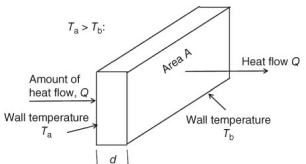
\includegraphics[width=0.68\linewidth]{slab}
		\caption{Conduction of heat in a solid slab}
		\label{fig:4_1}
	\end{figure}
	The natural phenomenon of that heat flow in a substance is possible only in the presence of temperature
	gradients, with heat flowing from locations at higher temperature to locations at lower temperature.
	Consequently, heat will flow from the left side to the right side of the slab if we maintain a state of $T_a > T_b$ with $T_a$ and $T_b$ being the temperature at the left and right faces of the slab, respectively as in figure \ref{fig:4_1}. Mathematically, one may express the above qualitative correlations in the following form
	\begin{eqnarray}
		Q = k \frac{A(T_a - T_b)t}{d}\label{eq:4_10}
	\end{eqnarray}
	where the constant $k$ is the thermal conductivity of the solid.\sps
	Equation \refx{4_10} provides us with a way to relate the total heat flow in a planar slab with the temperature gradient $\Delta T = T_a - T_b$. A more realistic characterization of heat flow in solids is in terms of heat flux $q$, defined as the \textit{heat flow per unit area and time}. Thus, from \refx{3_10}, we may express the heat flux in the slab as
	\begin{eqnarray}
		q = \frac{Q}{At} = k\frac{(T_a - T_b)}{d}\label{eq:4_11}
	\end{eqnarray}
	The heat flux across the two faces separated by the "thickness`` $\Delta x $ can be expressed as
	\begin{eqnarray}
		q = k\frac{T(x) - T(x + \Delta x)}{\Delta x} = -k\frac{T(x+\Delta x) - T(x)}{\Delta x}\label{eq:4_12}
	\end{eqnarray}
	Since the temperature variation in the slab varies as a continuous function $T(x)$ with $\Delta\to 0$, we have the following relation for the continuous variation of function $T(x)$ with the variable $x$
	\begin{eqnarray}
		q = q(x) = -k\frac{dT(x)}{dx}\label{eq:4_13}
	\end{eqnarray}
	where the temperature gradient is $\Delta T = T(x+\Delta x) - T(x)$ with $\Delta x \to 0$. Equation \refx{4_13} is the mathematical form of Fourier's law of heat conduction in one-dimensional heat flow along the coordinate $x$. One can recognizes this law as a first-order differential equation for the rate of change of temperature in a solid in the direction along the positive x-coordinate.
	
	\eg
	A 1 meter long metal rod is thermally insulated around its circumference. The terminal temperatures of the rod are measured to be $100^{\circ}C$ and $20^{\circ}C$. Determine the heat flux in the rod for the cases where it is made of copper and of aluminium.
	\begin{figure}[h!]
		\centering
		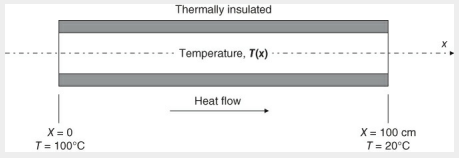
\includegraphics[width=0.8\linewidth]{heatflow}
	\end{figure}
	{~}\spn{-1.3}
	\solution
	The thermal conductivities (k) for copper and aluminium are $k_{cu}=3.95W/cm-^{\circ}C$ and $k_{Ai} = 2.36W/cm-^{\circ}C$, respectively. \sps
	The differential equation for the problem can be expressed slightly as
	\begin{equation}
		\frac{dT(x)}{dx} = - \frac{q}{k_{cu}} = -\frac{q}{3.95}\tag{a}\label{t:a_1}
	\end{equation}
	and the appropriate boundary condition is given by
	\begin{eqnarray*}
		T(0) = 100^{\circ}C
	\end{eqnarray*}
	The solution of the first-order differential equation in \refn{t:a_1} is given by
	\begin{equation*}
		T(x) = -\frac{q}{3.95}x + c
	\end{equation*}
	where $c$ is the integration constant. Now, using the first boundary condition, we have
	\begin{equation}
		T(x) = -\frac{q}{3.95}x + 100\tag{b}\label{t:b_1}
	\end{equation}
	Using the second boundary $T(100)=20^{\circ}C$, we get the heat flux $q$ from \refn{t:b_1} as
	\begin{eqnarray*}
		q = 3.16 W/cm^2
	\end{eqnarray*}
	Following the same procedure we find the corresponding heat flux in an aluminium rod to be $1.89 W/cm^2$.
	
	\section{RIGID BODY DYNAMICS}
	In this section, we will demonstrate how the first-order differential equations for rigid body dynamics analysis under the influence of gravitation can be derived using Newton's second law.\\
	
	\NI Consider a rigid body of mass $m$ that is thrown vertically up into the air with an initial velocity $v_0$, or that is falling from some height above the ground. 
	\begin{figure}[h!]
		\centering
		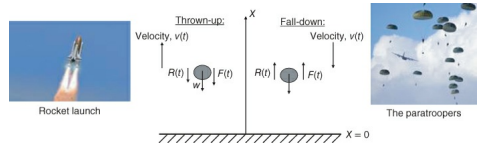
\includegraphics[width=0.9\linewidth]{rigid}
		\caption{Rise and fall of rigid bodies}
		\label{fig:4_2}
	\end{figure}
	The moving body encounter air resistance, which is proportional to the velocity $v(t)$, with $t$ being the time into the motion, we may derive the following equations:
	\begin{enumerate}
		\renewcommand{\labelenumi}{\alph{enumi}}
		\item The equation of motion in the coordinate systems as shown in figure \ref{fig:4_2}
		\item An expression for the velocity of the mass at time $t$
		\item The time at which the rigid body reaches its maximum height with an initial velocity in the case of the body thrown up, or the velocity at the touchdown for the body falling from an initial height.
	\end{enumerate}
	Newton's law on dynamic force equilibrium, $\sum F_x = 0$ is used to derived the differential equation from the force diagram shown at the left side of figure \ref{fig:4_2} when a body thrown up under the influence of gravitation
	\begin{eqnarray}
		\sum F_x = -F(t) - w - R(t) = 0\label{eq:4_14}
	\end{eqnarray}
	bearing in mind that both $R(t)$ and $F(t)$ act on the moving body in the direction opposite to that of the motion.\sps
	Now, substituting $R(t) = cv(t)$ and $F(t)=ma=mdv(t)$ into the above expression \refx{4_14}, we obtain the differential equation for the instantaneous velocity of the moving body
	\begin{eqnarray}
		\frac{dv(t)}{dt} + \frac{c}{m}v(t) = -g\label{eq:4_15}
	\end{eqnarray}
	The solution to the differential equation \refx{4_15} can be obtained using the linear differential equation technique.
	
	\NI Comparing \refx{4_15} with \refx{2_28}, we have
	\begin{eqnarray}
		P(t) = \frac{c}{m}\qquad\text{and}\qquad Q(t) = -g\label{eq:4_16}
	\end{eqnarray}	
	The integrating factor is given by
	\begin{eqnarray}
		IF = e^{\int c/m dt} = e^{ct/m}  \label{eq:4_17}
	\end{eqnarray}
	Thus, we have
	\begin{eqnarray}
		v(t) &=& \frac{1}{e^{ct/m}}\int e^{ct/m}(-g)dt +Ke^{-ct/m}\label{eq:4_18}
	\end{eqnarray}
	Now, consider the integral part of \refx{4_18}, i.e
	\begin{eqnarray}
		\int e^{ct/m}(-g)dt\label{eq:4_19}
	\end{eqnarray}
	Let
	\begin{eqnarray}
		u = \frac{c}{mc}\notag\sps
		\Rightarrow \frac{du}{dt} = \frac{c}{m}\notag\sps
		\Rightarrow \frac{mdu}{c} = dt\label{eq:4_20}
	\end{eqnarray}
	Putting the value of the $dt$ from \refx{4_20} in the integral \refx{4_19}, we get
	\begin{eqnarray}
		\int e^{ct/m}(-g)dt &=& \int e^u\notag \frac{mdu}{c}\sps
		\int e^{ct/m}(-g)dt&=& \frac{m}{c}\int e^u du\notag\sps
		\int e^{ct/m}(-g)dt&=& \frac{m}{c}e^u\label{eq:4_21}
	\end{eqnarray}
	Now, replacing the integral in \refx{4_18} with \refx{4_21}, thus equation \refx{4_18} becomes
	\begin{eqnarray*}
		v(t) &=& \frac{-g}{e^{ct/m}} \cdot \frac{c}{m}e^{ct/m}+ Ke^{-ct/m}
	\end{eqnarray*}
	which simplifies to
	\begin{eqnarray}
		v(t) &=& -\frac{mg}{c} + Ke^{-ct/m}
	\end{eqnarray}
	And this is the required solution to the given differential equation. Where $K$ is constant to be determined from an appropriate initial condition.\sps
	
	\NI For a given initial condition that $v(0) = v_0$, one may compute $K=v_0 + (mg/c)$. This will lead to the complete solution of $v(t)$ as 
	\begin{eqnarray}
		v(t) = -\frac{mg}{c} +\left(v_0\frac{mg}{c}\right)e^{-ct/m}\label{eq:4_23}
	\end{eqnarray}
	Equation \refx{4_23} gives the instantaneous velocity of a rigid body thrown upward with initial velocity of $v_0$.\sps
	
	\NI The time for the body to reach the maximum height, $t_m$ can be obtained by letting the velocity in equation \refx{4_23} be zero at that instant, i.e $v(t_m)=0$. The following relation derived from equation \refx{4_23} is used to obtain $t_m$
	\begin{eqnarray*}
		0 = -\frac{mg}{c}+\left(v_0\frac{mg}{c}\right)e^{-ct/m}
	\end{eqnarray*}
	Thus, from above equation, $t_m$ is given by
	\begin{eqnarray}
		t = \frac{m}{c}\ln\left(1 + \frac{v_0 c}{mg}\right)
	\end{eqnarray}

	%%%%%%%%%%%%%%%%%%%CHAPTER FIVE%%%%%%%%%%%%%%%%%%%
	\chapter{SUMMARY, CONCLUSION AND RECOMMENDATION}
	\section{SUMMARY}
	In this project, chapter one provided a general introduction to differential equations with related motivations and concepts.\\
	
	\NI Chapter two was used to elaborate on types, methods, and examples of first order differential equation and\\
	
	\NI A brief account of some first application of differential equation to biological, mechanical and electrical engineering were presented and solved in chapter three and four.
	
	
	\section{CONCLUSION}
	The most important branch of mathematics used for mathematical formulation is the differential equation.  Any physical situation involved motion or measure rates of change can be described by a mathematical model, the model is just a differential equation.This equation effectively related the quality or function upon which the attention is focused with the independent variable such as time, position upon which it may depend. Thus, the study of ordinary differential equation cannot be ignored and in this project, we were able to solved some biological and engineering problems using ordinary differential equation.\\
	
	
	\section{RECOMMENDATION}
	The application of differential equation in biological, mechanical and electrical engineering is recommended for organizations such as ministry of health, work and non-governmental organization. The area is fertile in terms of research and we therefore recommend students and researchers to venture into this area. Consequently, the government of Nigeria should also look into this area and motivate people in it.  
	
	
	%%%%%%%%%%%%%%%%%%%REFERENCE%%%%%%%%%%%%%%%%%%%
	\chapter*{REFERENCES}
	\addcontentsline{toc}{chapter}{REFERENCES}
	
	\begin{description}
		\item Adesola O. Anidu, Samson A. Arekete, Ayomide O. Adedayo \& Adekunle O. Adekoya (2015). \emph{Dynamic Computation of Runge-Kutta’s Fourth-Order Algorithm for
		First and Second Order Ordinary Differential Equation Using Java}. IJCSI International Journal of Computer Science Issues, Volume 12, Issue 3, May 2015 ,ISSN (Print): 1694-0814 | ISSN (Online): 1694-0784.
		
		\item Arfken, G.(1985). \emph{Self-Adjoint Differential Equations}. Mathematical Methods for Physicists,3rd ed.; Academic Press: Orlando, FL, USA, ; pp. 497–509.
		
		\item Atkinson K, Han W, Stewart D, (2009). \emph{Numerical Solution of Ordinary Differential Equations}. New Jersey: John Wiley \& Sons, Hoboken: 70-87.
		
		\item Bernoulli, \& John. \emph{Acta erunditorum}., Ostwald's Klassiker, No. 46. Engelmann,
		Leipzig, 1894.
		
		\item Butcher, J. (2003). \emph{Numerical Methods for Ordinary Differential Equations}. West Sussex:
		John Wiley \& Sons Ltd. 45-95.
		
		\item Dass, H. K. (1988). \emph{Advanced Engineering Mathematics} (1st ed., pp. 154–230). S. CHAND \& COMPANY PVT. LTD.
		
		\item Frank Ayres (1952). \emph{Schum's Outline Series, Theory and Problems of Differential Equations}. McGraw-Hill.
		
		\item Frank Hoppensteadt (1995). \emph{Getting Started to Mathematical Biology}. The American Mathematical Society. \\ https://www.ams.org/notices/199509/hoppensteadt.pdf
		
		\item Gentry R.D (1978). \emph{Introduction to Calculus for The Biological and Health Sciences}, Addition (Wesley Publishing Company).
		
		\item G. William (1973). \emph{An Introduction to Electrical Circuit Theory}. Red Globe Press London.
		\\https://doi.org/10.1007/978-1-349-03637-0
		
		\item Ince E.L (1956). \emph{Ordinary Differential Equations}, (1st Edition). Dover Publications, Inc., New York.
		
		\item Islam, Md.A. (2015a). \emph{Accuracy Analysis of Numerical solutions of Initial Value
		Problems (IVP) for Ordinary Differential Equations (ODE)}. IOSR Journal of Mathematics, 11, 18-23.
	
		\item Islam, Md.A. (2015b). \emph{Accurate Solutions of Initial Value Problems for Ordinary Differential Equations with Fourth Order Runge-Kutta Method}. Journal of Mathematics Research, 7, 41-45. \\http://dx.doi.org/10.5539/jmr.v7n3p41
		
		\item Leigh E.R (1968). The Ecological Role of Volterra’s Equation In Lectures On Mathematics In The Life Science Some Mathematical Problems In Biology.
		
		\item Lotka, A. J. (1957). \emph{Elements of Mathematical Biology}. New York, N. Y.: Dover Publisher. \\
		https://doi.org/10.1604/9780486603469
		
		\item Riley, K. F. (2012). Mathematical Methods for the Physical Sciences. \emph{An Informal Treatment for Students of Physics and Engineering}.\\ https://doi.org/10.1017/CBO9781139167550
		
		\item Ritger, P. D., \& Rose, N. J. (2010). \emph{Differential Equations with Applications}. Dover Publications.
		
		\item Rainville, E., Bedient, P., \& Bedient, R. (1996). \emph{Elementary Differential Equations}. Pearson. https://doi.org/10.1604/9780135080115.		
		
		\item Stroud, K. A., \& Booth, D. J. (2013). \emph{Engineering Mathematics}(7th Edition). \\ https://doi.org/10.1057/978113703122810.1057/978-1-137-03122-8
		
		\item Thomas A.B \& Finney, R. (1988). Calculus and Analytic Geometry 7th Editions. Reading Addison Wesley.
	\end{description}
	
\end{document}